	\subsection{UC 5 - Gestione dispositivi}
		
		\begin{figure}[H]
			\centering
			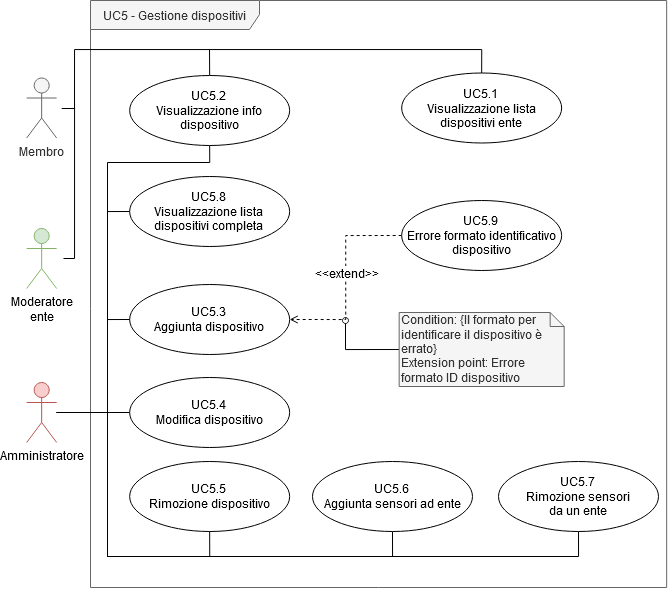
\includegraphics[scale=0.60]{res/images/uc5}
			\caption{Diagramma che riassume la gestione dei dispositivi all'interno della web app.}
		\end{figure}
		
		\begin{itemize}
			\item \textbf{Attori Primari}: Membro, Moderatore ente, Amministratore.
			\item \textbf{Descrizione}: L'utente può gestire i dispositivi a cui ha accesso a livello di permessi ed eseguire aggiunte, modifiche o rimozioni.
			\item \textbf{Precondizione}: L'utente è autenticato e naviga nella gestione dispositivi del sistema.
			\item \textbf{Postcondizione}: L'utente ha visualizzato o gestito i dispositivi.
			\item \textbf{Scenario Principale}:
			\begin{enumerate}
				\item{L'utente naviga all'interno della gestione dispositivi del sistema;}
				\item{L'utente visualizza o gestito i dispositivi a cui ha accesso.}
			\end{enumerate}
		\end{itemize}
			
			
			\subsubsection{UC 5.1 - Visualizzazione lista dispositivi ente}
			\begin{itemize}
				\item \textbf{Attori Primari}: Membro, Moderatore ente.
				\item \textbf{Descrizione}: L'utente può visualizzare i dispositivi abilitati per il proprio ente.
				\item \textbf{Precondizione}: L'utente naviga nella gestione dispositivi del sistema.
				\item \textbf{Postcondizione}: L'utente ha visualizzato i dispositivi.
				\item \textbf{Scenario Principale}:
				\begin{enumerate}
					\item{L'utente visualizza i dispositivi abilitati per il proprio ente}
				\end{enumerate}
			\end{itemize}
			
			\subsubsection{UC 5.2 - Visualizza info dispositivo}
			\begin{itemize}
				\item \textbf{Attori Primari}: Membro, Moderatore Ente, Amministratore.
				\item \textbf{Descrizione}: L'utente può visualizzare le informazioni riguardanti il dispositivo selezionato.
				\item \textbf{Precondizione}: L'utente naviga nella gestione dispositivi del sistema.
				\item \textbf{Postcondizione}: L'utente ha visualizzato le informazioni del dispositivo selezionato.
				\item \textbf{Scenario Principale}:
				\begin{enumerate}
					\item{L'utente seleziona il dispositivo dalla lista dispositivi;}
					\item{L'utente visualizza le informazioni del dispositivo.}
				\end{enumerate}
			\end{itemize}
			
			\subsubsection{UC 5.3 - Aggiunta dispositivo}
			\begin{itemize}
				\item \textbf{Attori Primari}: Amministratore
				\item \textbf{Descrizione}: L'utente può aggiungere, e quindi censire, un nuovo dispositivo nel sistema.
				\item \textbf{Precondizione}: L'utente naviga nella gestione dispositivi del sistema.
				\item \textbf{Postcondizione}: L'utente ha aggiunto un nuovo dispositivo al sistema.
				\item \textbf{Scenario Principale}:
				\begin{enumerate}
					\item{L'utente deve inserire dei campi obbligatori per aggiungere un nuovo dispositivo;}
					\item{L'utente compila il campo \textit{identificativo dispositivo} (UC 5.3.1);}
					\item{L'utente compila il campo \textit{nome dispositivo} (UC 5.3.2);}
					\item{L'utente compila il campo \textit{tempo di frequenza ricezione dati} (UC 5.3.3);}
					\item{L'utente compila il campo \textit{dati sensori}( UC 5.3.4); }
					\item{L'utente ha aggiunto un nuovo dispositivo al sistema.}
				\end{enumerate}
				\item \textbf{Estensioni}:
				\begin{itemize}
					\item Dispositivo non valido (UC 5.9)
				\end{itemize}
			\end{itemize}

				\paragraph{UC 5.3.1 - Inserimento identificativo dispositivo}
				\begin{itemize}
					\item \textbf{Attori Primari}: Amministratore
					\item \textbf{Descrizione}: Per proseguire nella aggiunta di un nuovo dispositivo, l'utente deve inserire l'identificativo del dispositivo. Il campo è obbligatorio.
					\item \textbf{Precondizione}: L'utente sta inserendo le informazioni per aggiungere un nuovo dispositivo.
					\item \textbf{Postcondizione}: L'utente ha compilato un campo richiesto.
					\item \textbf{Scenario Principale}:
					\begin{enumerate}
						\item{L'utente compila il campo \textit{identificativo dispositivo};}
					\end{enumerate}
				\end{itemize}

				\paragraph{UC 5.3.2 - Inserimento nome dispositivo}
				\begin{itemize}
					\item \textbf{Attori Primari}: Amministratore
					\item \textbf{Descrizione}: Per proseguire nella aggiunta di un nuovo dispositivo, l'utente deve inserire un nome con cui associare il dispositivo. Il campo è obbligatorio.
					\item \textbf{Precondizione}: L'utente sta inserendo le informazioni per aggiungere un nuovo dispositivo.
					\item \textbf{Postcondizione}: L'utente ha compilato un campo richiesto.
					\item \textbf{Scenario Principale}:
					\begin{enumerate}
						\item{L'utente compila il campo \textit{nome dispositivo};}
					\end{enumerate}
				\end{itemize}

				\paragraph{UC 5.3.3 - Inserimento tempo di frequenza ricezione dati}
				\begin{itemize}
					\item \textbf{Attori Primari}: Amministratore
					\item \textbf{Descrizione}: Per proseguire nella aggiunta di un nuovo dispositivo, l'utente deve inserire il tempo di frequenza per la ricezione dati nel sistema. Il campo è obbligatorio.
					\item \textbf{Precondizione}: L'utente sta inserendo le informazioni per aggiungere un nuovo dispositivo.
					\item \textbf{Postcondizione}: L'utente ha compilato un campo richiesto.
					\item \textbf{Scenario Principale}:
					\begin{enumerate}
						\item{L'utente compila il campo \textit{tempo di frequenza ricezione dati};}
					\end{enumerate}
				\end{itemize}

				\paragraph{UC 5.3.4 - Inserimento dati sentori}
				\begin{itemize}
					\item \textbf{Attori Primari}: Amministratore
					\item \textbf{Descrizione}: Per proseguire nella aggiunta di un nuovo dispositivo, l'utente deve inserire i dati dei sensori del dispositivo di cui vuole ricevere letture. Il campo è obbligatorio.
					\item \textbf{Precondizione}: L'utente sta inserendo le informazioni per aggiungere un nuovo dispositivo.
					\item \textbf{Postcondizione}: L'utente ha compilato un campo richiesto.
					\item \textbf{Scenario Principale}:
					\begin{enumerate}
						\item{L'utente compila il campo \textit{dati sensori};}
					\end{enumerate}
				\end{itemize}

			
			\subsubsection{UC 5.4 - Modifica dispositivo}
			\begin{itemize}
				\item \textbf{Attori Primari}: Amministratore.
				\item \textbf{Descrizione}: L'utente modifica i dispositivi che gli interessano e la nuova configurazione viene gestita dal sistema.
				\item \textbf{Precondizione}: L'utente naviga nella gestione dispositivi del sistema e ha almeno un dispositivo disponibile.
				\item \textbf{Postcondizione}: L'utente ha modificato il dispositivo selezionato.
				\item \textbf{Scenario Principale}:
				\begin{enumerate}
					\item{L'utente seleziona un dispositivo da modificare;}
					\item{L'utente modifica il campo \textit{nome dispositivo} (UC 5.4.1);}
					\item{L'utente modifica il campo \textit{tempo di frequenza ricezione dati} (UC 5.4.2);}
					\item{L'utente modifica i \textit{dati sensori} (UC 5.4.3);}
					\item{L'utente ha modificato il dispositivo selezionato.}
				\end{enumerate}
			\end{itemize}

			% ndr: da come ha detto Alex, sarebbe da fare una roba che prima modifica tutti i dispositivi e poi c'è un tasto di conferma una volta che tutto è stato modificato. A livello DB si può aggiungere una tabella per gestire i dispositivi modificati e poi controllare quando è stata sovrascritta l'ultima configurazione a un gateway.
			
				\paragraph{UC 5.4.1 - Modifica nome dispositivo}
				\begin{itemize}
					\item \textbf{Attori Primari}: Amministratore
					\item \textbf{Descrizione}: Per proseguire nella modifica di un dispositivo, l'utente deve modificare il nome con cui associare il dispositivo. Il campo è obbligatorio.
					\item \textbf{Precondizione}: L'utente sta modificando le informazioni di dispositivo già censito.
					\item \textbf{Postcondizione}: L'utente ha compilato un campo richiesto.
					\item \textbf{Scenario Principale}:
					\begin{enumerate}
						\item{L'utente compila il campo \textit{nome dispositivo};}
					\end{enumerate}
				\end{itemize}

				\paragraph{UC 5.4.2 - Modifica tempo di frequenza ricezione dati}
				\begin{itemize}
					\item \textbf{Attori Primari}: Amministratore
					\item \textbf{Descrizione}: Per proseguire nella modifica di un dispositivo, l'utente deve modificare il tempo di frequenza per la ricezione dati nel sistema. Il campo è obbligatorio.
					\item \textbf{Precondizione}: L'utente sta modificando le informazioni di dispositivo già censito.
					\item \textbf{Postcondizione}: L'utente ha compilato un campo richiesto.
					\item \textbf{Scenario Principale}:
					\begin{enumerate}
						\item{L'utente compila il campo \textit{tempo di frequenza ricezione dati};}
					\end{enumerate}
				\end{itemize}

				\paragraph{UC 5.4.3 - Modifica dati sensori}
				\begin{itemize}
					\item \textbf{Attori Primari}: Amministratore
					\item \textbf{Descrizione}: Per proseguire nella modifica di un dispositivo, l'utente deve modificare ildati dei sensori del dispositivo di cui vuole ricevere letture. Il campo è obbligatorio.
					\item \textbf{Precondizione}: L'utente sta modificando le informazioni di dispositivo già censito.
					\item \textbf{Postcondizione}: L'utente ha compilato un campo richiesto.
					\item \textbf{Scenario Principale}:
					\begin{enumerate}
						\item{L'utente compila il campo \textit{dati sensori};}
					\end{enumerate}
				\end{itemize}
			
			\subsubsection{UC 5.5 - Rimozione dispositivo}
			\begin{itemize}
				\item \textbf{Attori Primari}: Amministratore.
				\item \textbf{Descrizione}: L'utente può rimuovere dal sistema un dispositivo in base ai dispositivi censiti a sistema.
				\item \textbf{Precondizione}: L'utente naviga nella gestione dispositivi del sistema e ha almeno un dispositivo disponibile.
				\item \textbf{Postcondizione}: L'utente ha rimosso il dispositivo selezionato dal sistema.
				\item \textbf{Scenario Principale}:
				\begin{enumerate}
					\item{L'utente seleziona un dispositivo da rimuovere tra quelli disponibili;}
					\item{L'utente ha rimosso il dispositivo selezionato dal sistema.}
				\end{enumerate}
			\end{itemize}
			
			\subsubsection{UC 5.6 - Aggiunta sensori ad ente}
			\begin{itemize}
				\item \textbf{Attori Primari}: Amministratore.
				\item \textbf{Descrizione}: L'utente può aggiungere i permessi di lettura e monitoraggio dei dati di un dispositivo a un particolare ente.
				\item \textbf{Precondizione}: L'utente naviga nella gestione dispositivi del sistema.
				\item \textbf{Postcondizione}: L'utente ha concesso il monitoraggio di un sensore ad un ente.
				\item \textbf{Scenario Principale}:
				\begin{enumerate}
					\item{L'utente seleziona un sensore di un particolare dispositivo e lo abilita a un ente}
					\item{L'utente ha permesso il monitoraggio del sensore all'ente selezionato}
				\end{enumerate}
			\end{itemize}
			
			\subsubsection{UC 5.7 - Rimozione sensori da un ente}
			\begin{itemize}
				\item \textbf{Attori Primari}: Amministratore.
				\item \textbf{Descrizione}: L'utente può rimuovere i permessi di monitoraggio dei dati del dispositivo selezionato all'ente selezionato.
				\item \textbf{Precondizione}: L'utente visualizza le informazioni del dispositivo.
				\item \textbf{Postcondizione}: L'utente ha rimosso il permesso di monitoraggio del dato del dispositivo all'ente selezionato.
				\item \textbf{Scenario Principale}:
				\begin{enumerate}
					\item{L'utente rimuove un sensore di un particolare dispositivo a un ente}
					\item{L'utente ha rimosso il permesso di monitoraggio del sensore all'ente selezionato}
				\end{enumerate}
			\end{itemize}

			\subsubsection{UC 5.8 - Visualizzazione lista dispositivi completa}
			\begin{itemize}
				\item \textbf{Attori Primari}: Amministratore.
				\item \textbf{Descrizione}: L'utente può visualizzare la lista dei dispositivi completa.
				\item \textbf{Precondizione}: L'utente naviga nella gestione dispositivi del sistema.
				\item \textbf{Postcondizione}: L'utente ha visualizzato la lista di tutti i dispositivi.
				\item \textbf{Scenario Principale}:
				\begin{enumerate}
					\item{L'utente visualizza tutti i dispositivi presenti nel sistema.}
				\end{enumerate}
			\end{itemize}

			\subsubsection{UC 5.9 - Errore formato identificativo dispositivo}
			\begin{itemize}
				\item \textbf{Attori Primari}: Amministratore.
				\item \textbf{Descrizione}: L'utente visualizza un errore che segnala che il campo identificativo di un dispositivo non è valido.
				\item \textbf{Precondizione}: L'utente ha inserito un formato dell'identificativo di dispositivo errato.
				\item \textbf{Postcondizione}: L'utente visualizza un errore specifico.
				\item \textbf{Scenario Principale}:
				\begin{enumerate}
					\item Il sistema sta elaborando la richiesta;
					\item Viene visualizzato un errore che spiega che il formato utilizzato per l'identificativo del dispositivo non è corretto.
				\end{enumerate}
			\end{itemize}